\section{Strategy Improvements}\label{ch:strategy}

\subsection{Decision Tree}\label{subsec:decisionTree}
If the agent loses a level and re-enters it again at a later point of the competition, it should not try the same consecutive shots, that lead to failure in the first try, again. In order for the agent to gain knowledge about wether a shot led to failure or pass of a level, a decision tree was implemented (see \texttt{DecisionTree.class}). This way, the second, third or nth time the agent retries a level, it should not do the same bad shots over and over again. The decision tree is only of use in lost levels. It has no effect on levels that have already been won. It could, however, in future work be implemented so that if an already won level is retried, the agent will not do the exact same shots again, but try something new and see if it gets more points.

\subsubsection{Functionality of the decision tree}
Every time the agent enters a level for the very first time, a single instance of a tree is saved within the level representation of that level. Every time the agent re-enters a level, its already existent tree instance reloaded. Every time the level is being played, the same tree instance gets modified.

The root node of the tree is the situation the agent is in when it enters a level. Soon enough, Prolog calculates the options for the next shot and returns them to the agent. Each of those options represents a new node in the tree structure. The agent picks one of the options, shoots, and the respective node for that shot becomes the representation of the current situation and the node gets marked as \textit{visited}. Now, another set of possible next shots is calculated, new nodes are added and so on. In fig \ref{fig:take1}, the nodes on each level of the tree represent all options after one shot. The blue nodes represent shots that the agent decided to take, one after the other.

In the assumption that the last shot that is being conducted leads to losing the level, this node gets marked as \textit{lost} (see fig. \ref{fig:take1}). The tree is designed so that it never takes a shot that would lead to being in a situation that is marked as \textit{lost}. This means, that if one parent node has e.g. two childnodes, and, in a second attempt to win the level, both of them are lost, the parent node will also be marked as lost, as there is no way of winning the game if this node's shot is taken (see fig. \ref{fig:take2}).

\begin{figure}
	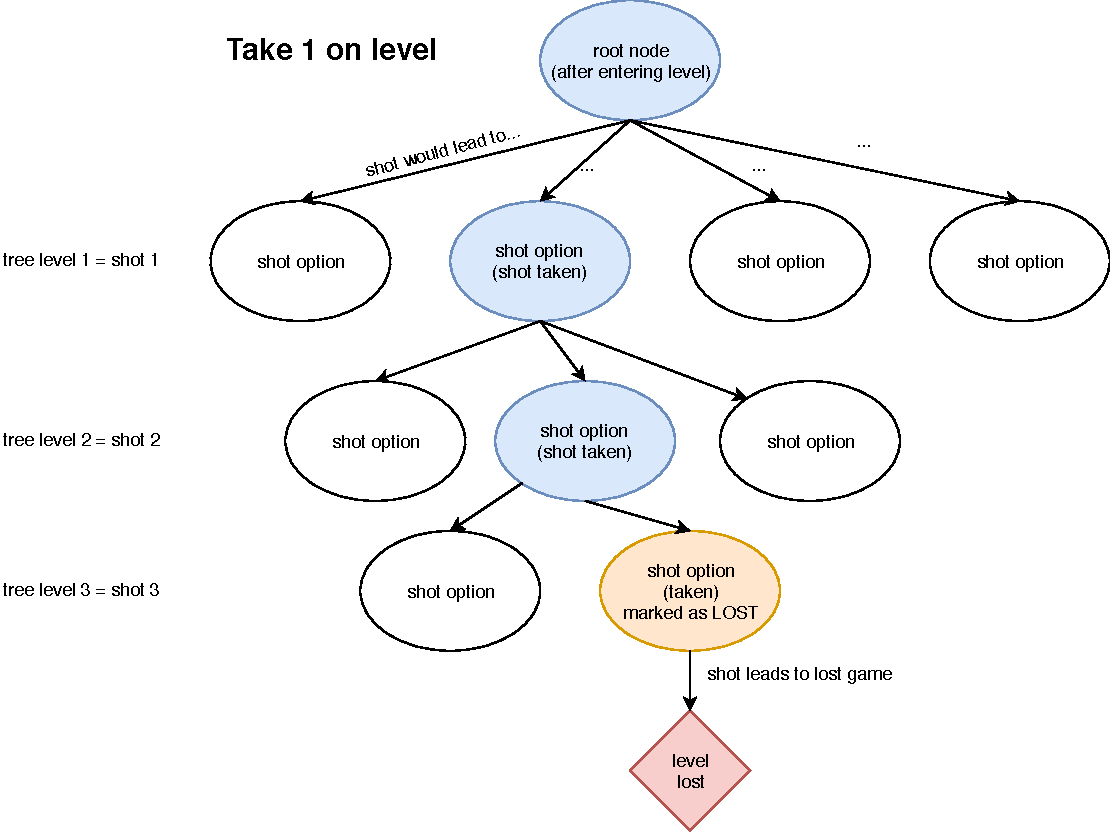
\includegraphics[width=\textwidth]{img/take1onlevel.pdf}
	\caption{First attempt to win the level ends with a lost game. The last node (which represents the shot that used the last bird) is marked as \textit{lost} and will never be taken again.}\label{fig:take1}
\end{figure}
\begin{figure}
	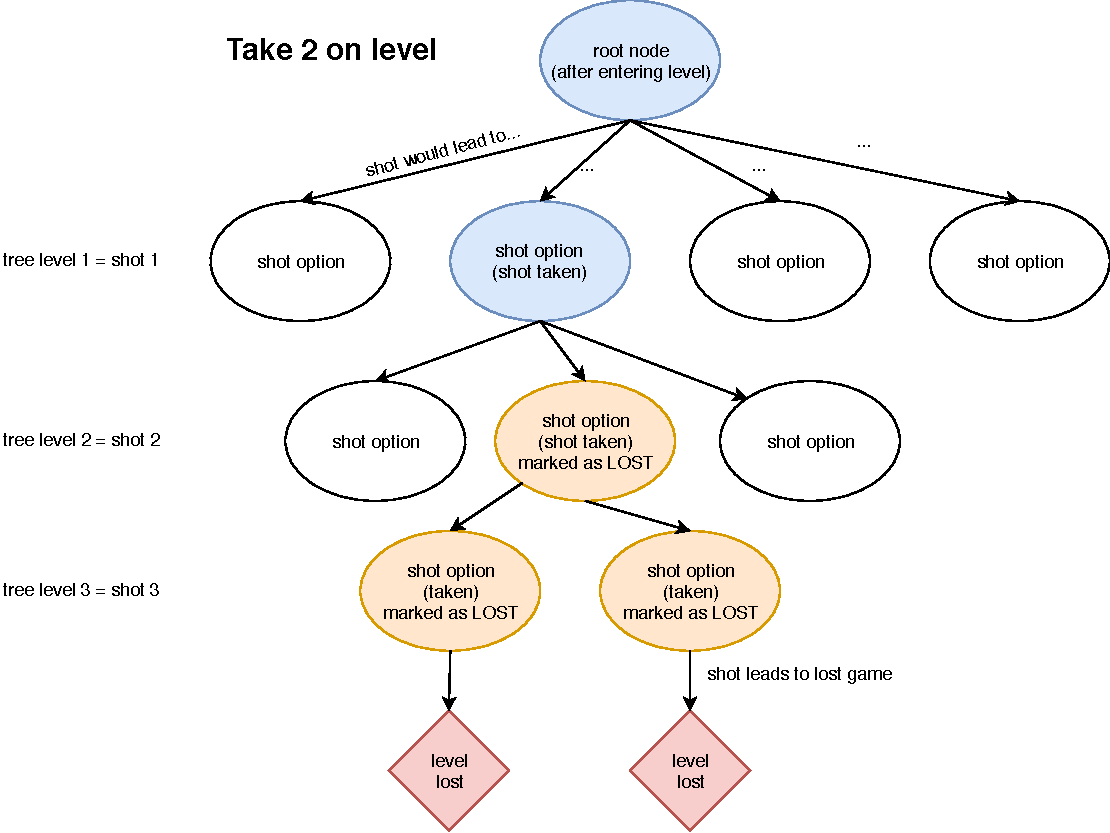
\includegraphics[width=\textwidth]{img/take2onlevel.pdf}
	\caption{In this example, the shot path in the second attempt stays largely the same. Since all two child nodes of the taken shot on level 2 led to lost games, the node on level 2 is also marked as lost.}\label{fig:take2}
\end{figure}

\subsubsection{Backpropagating negative impact for the confidence of a shot}\label{subsec:backpropagationConfidence}
Whenever Prolog calculates the options for the next shot, it provides the agent with a list with all possibly successful shots. Those possible shots all have a confidence rating, which expresses how successful Prolog predicts the shot would be. The agent currently picks its next shot according to the shot with the highest confidence rating. If a shot leads to a loss, we backpropagate a negative impact on this confidence all the way back to the root node for every shot that had been taken on the way to losing the game. This impact starts with \(-0.5\) for the parent of the lost node (see fig. \ref{fig:negativeImpact}. The impact is being divided by two for every node on the way back to the root node. This way, the agent will be encouraged to decide for a different chain of shots before it is in a situation that will likely lead to a loss again.

\begin{figure}
	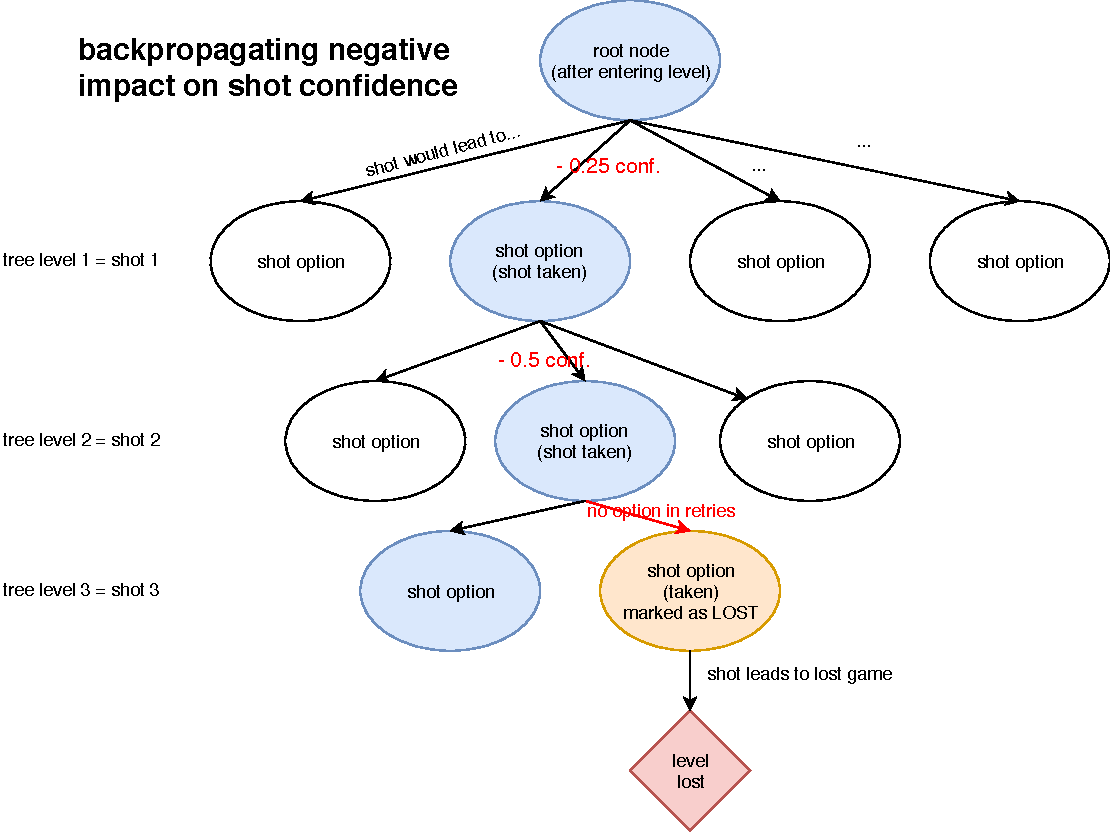
\includegraphics[width=\textwidth]{img/negImpact.pdf}
	\caption{Backpropagation of negative impact of a loss. The impact starts at the parent of the lost node, since the lost node itself will never be re-entered again anyway.}\label{fig:negativeImpact}
\end{figure}

\subsubsection{The problem of randomness in the physics of the game}\label{subsec:randomnessInPhysics}
If the agent enters a level twice, the same best shot is calculated twice and the same shot is taken twice, one would assume the level on the first attempt looks exactly the same as on the second attempt. However, there is a small randomness in Angry Birds' physics. This means that sometimes, when a level is entered for the second time, one can not be sure that if the same shot is taken, the tree would look the same as the first time. In order to prevent the tree representation of the game situation looking different than the actual game situation, after each taken shot, the current situation's screenshot is being compared to the screenshot of the previous attempt. If the level looks different despite having taken the same shot, the current situation will be saved in the tree inside a newly created node.

\subsubsection{Shots that have no effect}\label{subsec:shotsThatHaveNoEffect}
If the agent shoots e.g. onto a concrete terrain block, no damage is done by that shot. This means that the level will also still look the same. That shot then was completely wasted. In order to prevent the agent from taking repeatedly shots that do not change the situation, each time a shot is conducted, the situation after that shot will be compared (by comparing the blocks' positions) to the situation before the shot. If the level still looks the same, a new node will be appended to the current node that is marked as \textit{lost}. For every shot the agent takes, it checks beforehand if the current node has a child node containing the exact same shot. In this case, this would be true, and that node would also be marked as lost. This shot would then not be taken.

%The slope detection is on it's onw branch, and has not been merged with the master branch. 
%This is mostly due to a lack of testing.
\subsection{Slope Strategy}\label{subsec:slopeStrategy}
So far, the Agent has ignored "Heavy Objects", like large stone boulders, completely, excluding cases where they were directly above a 'priority target', aka a pig or TNT. Several Angry Birds levels contain such Boulders on the top of hills, or on a slope, blocked by a destructible object. The new slope detection checks several positions around boulders for contact with the ground, or a hill, and determines if the boulder in question could be made to roll down a hill. If so, the agent will treat it similarly to heavy objects above pigs or TNT. \linebreak
As there is no support for complex interactions, it will not check for priority targets to the left of heavy objects of hilltops, as the agent has no means to nudge a boulder to the left while shooting from the left, and pigs on the left of a hill can usually be hit directly.
\ref{fig:Dec_Tree}
The agent checks the position of heavy objects if the vision module reports that they are resting on a hill. It does so by checking for collision of the bottom left and bottom right of the boulder's bounding box, which the vision module provided, to check for uneven ground, then checks for ground contact to the left and right of the object to detect a hilltop position. 
\ref{fig:slopeEx}
Currently, the slope detection does not check for multiple objects between the Heavy Object and Priority Targets.
\begin{figure}
	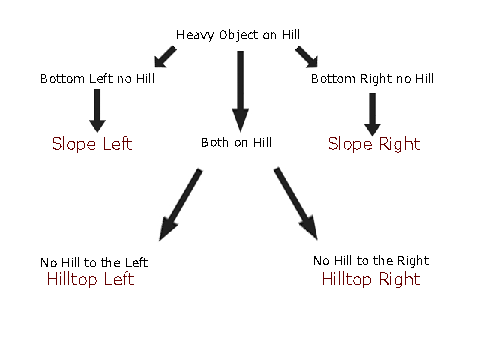
\includegraphics[width=\textwidth]{img/Dec_Tree.pdf}
	\caption{Decision tree to check for slopes. Heavy Objects on actual slopes do not need to check for hilltops in the same direction.}\label{fig:slopeEx}
\end{figure}

\begin{figure}
	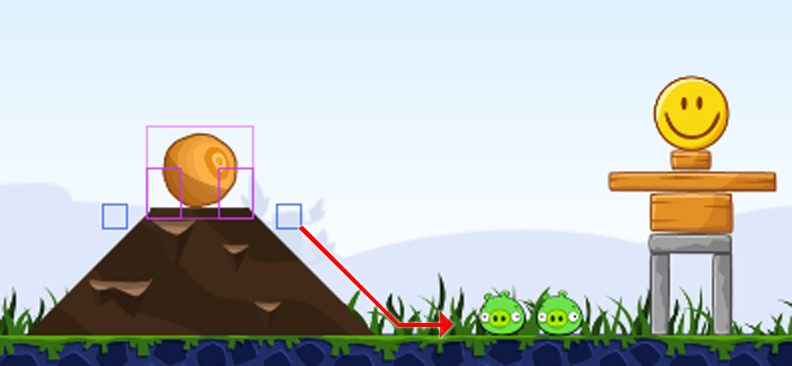
\includegraphics[width=\textwidth]{img/shot1hr}
	\caption{Slopecheck: The Heavy Object is sitting on a hilltop.  In this example, there is a priority target to the bottom right of the boulder, indicating the boulder as a potential target for a direct shot.}\label{fig:slopeEx}
\end{figure}

% this has not been implemented. It might be in the future though, after further evaluation.
\subsection{Weka Machine Learning \textit{not implemented yet}}
Disclaimer: this option of further improvement of the agent has not been implemented yet. It might be helpful in the future, though. Further investigation and evaluation is required. This chapter is just a description of current findings.

\subsubsection{Introduction}
Weka is a collection of machine learning algorithms for data mining tasks. It includes methods for data mining problems such as regression, classification, clustering, association rule mining, and attribute selection \footnote{Eibe Frank, Mark A. Hall, and Ian H. Witten (2016). The WEKA Workbench. Online Appendix for "Data Mining: Practical Machine Learning Tools and Techniques", Morgan Kaufmann, Fourth Edition, 2016.}. Weka is used by applying a learning algorithm to a given dataset and analyzing its output. Another way of using Weka, which is relevant for our use in BamBird agent, is to generate predictions on new instances, and a third way is to apply different learning algorithms and compare their outputs and performances.

\subsubsection{Implementation}
For the use in BamBird, Weka is used to classify a new instance. The class to be learned is whether a shot is good or bad, this is called a relation in Weka. This relation is dependent on attributes, and the attributes for the BamBird agent are, strategy name, confidence class, damage points and pigs killed. Weka uses an ARFF \footnote{https://www.cs.waikato.ac.nz/ml/weka/arff.html}. file. The ARFF file contains two sections, the header section and the data section. We give a brief description. Below we show the header of the ARFF file. The header contains the relation, a list of attributes and their data types.

The header section of the ARFF file looks like this:
\begin{lstlisting}
@relation good-shot
@attribute strategy-name 	{targetPig ,domino, blackBird,
collapseStructure, tnt, heavyObject, whiteBird}
@attribute confidence-class	{A, B, C}
@attribute damage-points	REAL
@attribute pigs-killed		REAL
@attribute class		{good, bad}
\end{lstlisting}
\ \\
The header section of the ARFF file is followed by the ARFF Data Section. It contains the data declaration line and the dataset. Below we show a snapshot of our training dataset. Default values from section 4.1 are used to mark a shot as good or bad. Confidence class is identified as follows: class A from 0.5 to 0.6, class B from 0.6 to 0.9 and class C from 0.9 to 1.0. The Data Section looks like this:

\begin{lstlisting}
@data

domino,C,0,0,bad
domino,C,0,0,bad
targetPig,C,8760,2,good
domino,C,16100,3,good
targetPig,C,5320,2,good
targetPig,C,12530,3,good
targetPig,A,1160,0,bad
targetPig,A,6440,2,good
heavyObject,C,32580,6,good
\end{lstlisting}
\ \\
In order to classify a new instance, a new ARFF file is created at runtime, called \texttt{unknown.arff}. The header of \texttt{unknown.arff} is the same as the header described above, but the data section is different. Instead of having an entire dataset, only one data is provided, described below.
\ \\
\ \\
\texttt{targetPig, A, ?, ?, ?}
\ \\
\ \\
The \texttt{?} is the dataset signifies unknown data. To classify this instance, we know that the strategy is \texttt{targetPig} and we know that the \texttt{confidence-class} is \texttt{A}, but \texttt{damage-points}, \texttt{pigs-killed} and shot \texttt{class} are unknown. We use the NaiveBayes algorithm as implemented by Weka to classify this new instance.
\ \\
\ \\
Following we present the updated \texttt{Meta} algorithm for Weka and the \texttt{ClassifyShot} algorithm.

\begin{algorithm}[H]
	\SetAlgoLined
	load the ShotLearner database\;
	\While{true}{
		\If{GameState != Playing}{
			choose new Level using the new equation\;
		}
		take a screenshot from the scene and analyse\;
		generate plans\;
		select the first Target from the plans and send it to WekaTester\;
		WekaTester classifyShot marks the Target good or bad\;
		\uIf{goodTarget}{
			execute the seleted shot\;
		} \uElse{
			remove the target from plan\;
			go to 8.\;
		}
		add shot to the shot-list of the current level\;
		\If{GameState == WON or GameState == LOST}{
			add level to database\;	
		}
		add the shot to ShotLearnerDatabase\;
		create a ShotResult object with the results of the shot\;
		save the ShotResult to a log file\;
	}
	\caption{Meta-Updated} \label{algorithm:metaUpdated}
\end{algorithm}
\ \\
Line 7 – 14 mark the difference in the updated \texttt{Meta} algorithm. A \texttt{Target} is selected from the generated list of plans and is sent to \texttt{WekaTester}, where this target is transformed into an instance and written to \texttt{unknown.arff} file.
\ \\
\ \\
\begin{algorithm}[H]
	\SetAlgoLined
	create unknown.arff file\;
	write the header\;
	transform target into ARFF data instance\;
	invoke NaiveBayes classifyInstance and save into prediction string\;
	return prediction string\;
	
	\caption{Weka: ClassifyShot}\label{algorithm:classifyShot}
\end{algorithm}
\ \\

There are two points of interest in Algorithm \ref{algorithm:classifyShot}. The first is the transformation of \texttt{Target} object into ARFF data instance. This is trivial and is achieved by string manipulation and string writing onto the \texttt{unknown.arff} file. The second interest point is the invoking of \texttt{classifyInstance} of \texttt{NaivesBayes} algorithm. This is also trivial because the logic is abstracted behind a simple method call, shown below.
\ \\
\ \\
\texttt{double predNB = nb.classifyInstance(newInst);} \footnote{http://weka.sourceforge.net/doc.stable/}
\ \\
\ \\
where \texttt{predNB } is the predicted class, \texttt{nb} is the instance of \texttt{NaiveBayes} class algorithm and newInst
is the new data instance that we wish to classify and predict the class of.
\ \\
\ \\
Implementing learning algorithms from Weka promise to be of use for the BamBird agent, but have not been implemented yet.
